
%---ARCHITECTURE---

\begin{wrapfigure}{r}{0.3\textwidth}
  \vspace{-50pt}
    \centering
    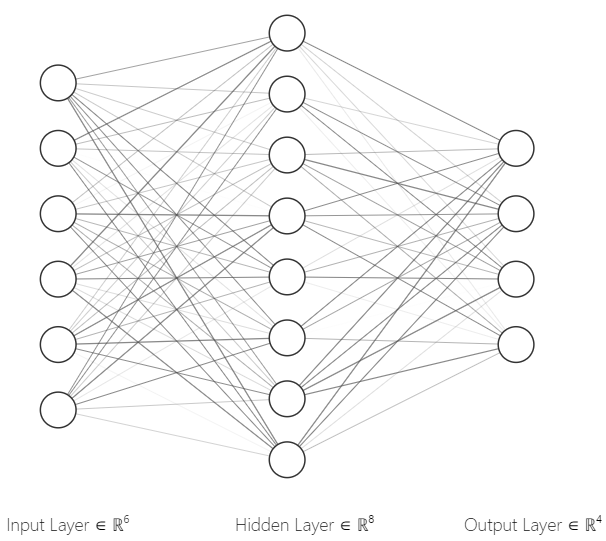
\includegraphics[width=.4\textwidth]{Figures/NN_int.png}
    \caption{\footnotesize{A two-layer neural network with the \emph{input} as the first layer and the \emph{hidden} layer as the second.  The final layer displayed is simply the output result}}
  \label{NNet}
  \vspace{-20pt}
\end{wrapfigure}

Artificial neural networks are composed of one or more layers in between the input data and the output results.  It is common for a $L$-layered network to be recognized as such by the number of $L$ layers that have tunable parameters; although some literature describes an alternate means of describing layer sizes \cite{bishop1995} (i.e. by counting the output layer rather than the input).  This thesis will only use the tunable weights criterion so not to confuse what the $l^{th}$ layer is referring to, as illustrated in Figure \ref{NNet}.  
A neural network is based on a feed-forward mapping, in which connections exist only directly between any two subsequent layers, and each unit (or \textit{neuron}) is connected to all neurons in its adjacent layer(s).  Such feed-forward designs are non-linear mappings between a set of input variables and a set of output variables, in which direct connections between layers are transformed by non-linear activation functions.\cite{bishop2006pattern}.
However, linearity can be achieved through the usage of a linear activation function.  In such cases, a linear neural network model is found to be more adaptive to data curvature, without the necessity for splines or higher order polynomials. \cite{?}
Indeed, a neural network devoid of any activation function simplifies to a linear regression model \ref{sharma2017activation}, which will be shown later in this section.


The Multi-Layer Perceptron (add these into this subsection)

\begin{itemize}
\tightlist
  
\item
  One hidden layer is sufficient to make accurate predictions from
  training data. More hidden layers increase the depth of the network,
  and often calls for fewer units per layer. Deeper networks are better
  at generalizing test data, but are harder to optimize
  \cite{Goodfellow-et-al-2016} \emph{(Re-address this claim down the
  road)}
\item 
    Hint toward issues like overfitting, but elaborate more later
\end{itemize}

\hypertarget{foundations}{%
\subsection{Foundations}\label{foundations}}

\textbf{The Perceptron} \textit{(bullet points to be converted into paragraph form)}

\begin{itemize}
\tightlist
\item
  artificial neuron developed by Frank Rosenblatt in the 1950s
  \cite{nielsen}
\item
  Takes several binary inputs and outputs a single binary output:
\item
  Output is determined by the weighted sum of all input values with
  respective weights
\end{itemize}

\[
Y = 
\begin{cases}
0 \text{ if } \sum_i^n w_ix_i \le D \\
1 \text{ if } \sum_i^n w_ix_i > D
\end{cases}
\] Where \(i\) can be any number \(n\) of input values composed in the
network and \(D\) is the threshold value that the weighted sum is
matched with to determine the binary output \(Y\).

Because these inputs are calculated by computers, and computers like
vectors, the notation is adjusted to allow for proper computation in which $(w_i \cdot x_i)$ is the \textit{dot product} of the weights and inputs. In
addition, Rosenblatt introduced a bias (check source) to shift the
function for a clean threshold of \(D = 0\). \[
Y = 
\begin{cases}
0 \text{ if } (w_i \cdot x_i) + b_i \le 0 \\
1 \text{ if } (w_i \cdot x_i) + b_i > 0
\end{cases}
\]

This is represented by the \emph{step function}.

\begin{figure}[H]
    \centering
    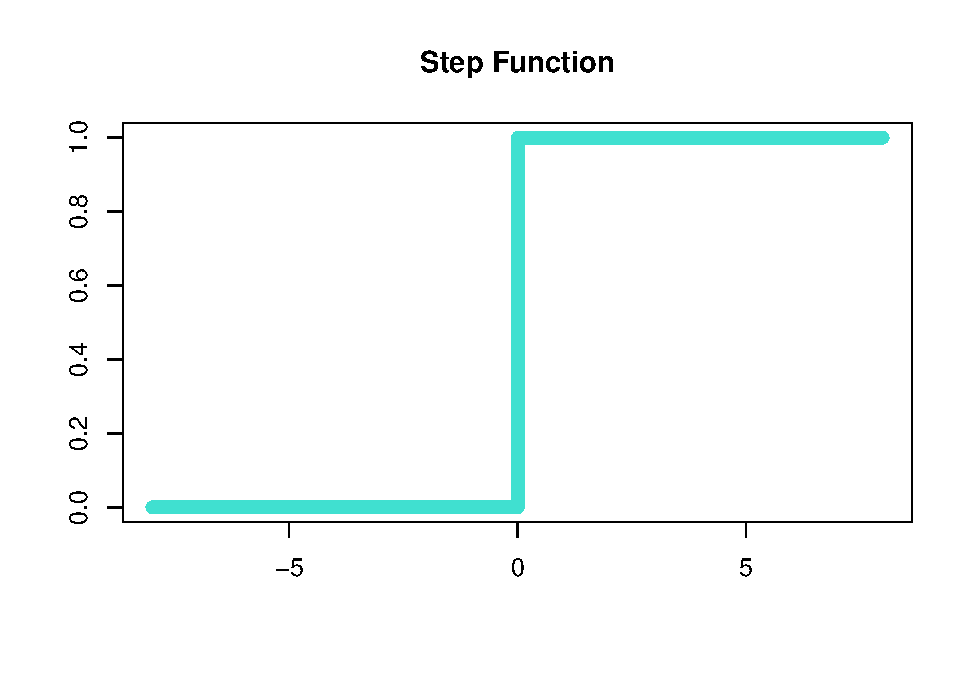
\includegraphics[width = .7\textwidth]{Figures/step-function-1.pdf}
    \vspace{-40pt}
 %   \caption{caption}
\end{figure}

The problem with the perceptron is that a small change in weight can
cause the outcome to change dramatically, since the output is binary.

\textbf{Sigmoid neuron}

The elementary topology of a neural network as featured in Figure \ref{NNet} is a \textbf{Multi-Layer Perceptron}.  Despite its name, it is typically composed of being composed of \textit{sigmoid neurons}.

\begin{itemize}
\tightlist
\item
  modified from perceptrons so that small changes in weights or bias
  causes a small change in output
\item
  not a binary output, rather an output of the interval {[}0,1{]}
\end{itemize}


\[
\sigma(z) = \frac{1}{1+e^{-z}} \\
\] Where \(z\) is the same equation from the perceptron
\(w \cdot x + b\). That is, 
$$
\sigma((w_i \cdot x_i) + b_i) = \frac{1}{1-e^{-((w_i \cdot x_i) + b_i)}}
$$

Which is represented by the \emph{Sigmoid Function}

\begin{figure}[H]
    \centering
    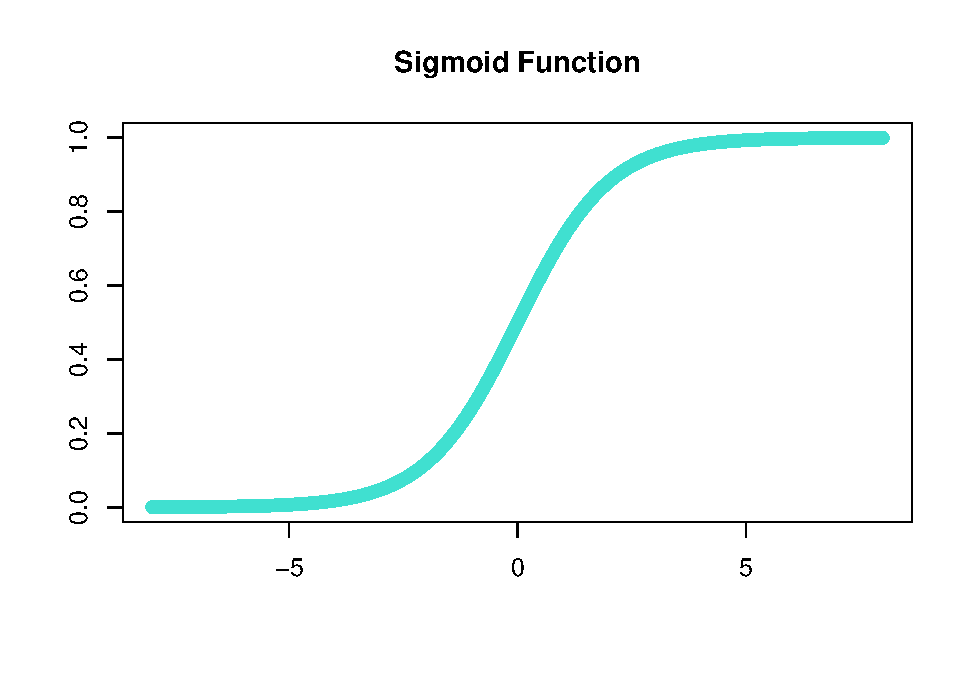
\includegraphics[width = .7\textwidth]{Figures/sigmoid-function-1.pdf}
   \vspace{-40pt}
%    \caption{caption}
\end{figure}

\textit{(So far this section has only dealt with connections in between two layers.  Continue here to connections into subsequent layers, including notation similar to Bishop 1995 p. 119)}

\textbf{A note on linearity}

A single-layer neural network would have but one step of calculations ($input \rightarrow output$).  With no hidden layer to perform subsequent calculations, the resulting interpretation would be the expected result of the given inputs.
$$
y_i = (w_i \cdot x_i) + b
$$
This means that a neural network devoid of any hidden layers or activation function simplifies to a \textbf{linear regression} model. \cite{sharma2017activation}


%In the case of a two-layer neural %network with no activation functions in %between:
%$$
%y_i = (w_{i2} \cdot ((w_{i1} \cdot %x_{i1}) + b_1)) + b_2
%$$


Similarly, it can also be noted that a neural network which uses the sigmoid activation function is a generalization of \textbf{logistic regression}. \cite{dreiseitl2002logistic} \cite{schumacher1996neural}  If $\delta$ denotes the logit function expressed as the log-odds of the outcome of $X$ (0 or 1):
$$
\delta = ln \left( \frac{P(X)}{1-P(X)} \right) = (w_i \cdot x_i) + b_i 
$$
Reversing $\delta$ results in the relevant probability that $X = 1$ for the given vector of weights and bias.
$$
P(X) = \frac{e^\delta}{1+e^\delta} = \frac{1}{1+e^{-\delta}}
$$
In which $P(X) \in [0,1]$.  For logistic regression, or for a single-layer neural network using the sigmoid activation function, the calculation would end here and the resulting interpretation from the binary classification model a probability that the input is from category 1.  In deeper neural networks, the value of $P(X)$, which is one of many, gets passed on to the next layer to join its cohorts for the next calculation.

The potential for neural networks expands well beyond linearity or the curvature matched by polynomial terms or splines.  Neural nets are universal function approximators, which means that they have the capacity to learn and compute any function. \cite{sharma2017activation} This is due to non-linear activation functions, for without them, transformations between successive layers would be linear, and the entire composition itself then linear, too. \cite{bishop1995}  While there is no one-size-fits all, certain activation functions have desirable properties that help give insight into the questions that neural networks answer.

%---------ACTIVATION FUNCTIONS---------

\hypertarget{activation-functions}{%
\subsection{Activation Functions}\label{activation-functions}}

A common theme of this thesis and neural network research in general is their immense complexity.  No feature of a neural network can be expressed in exhaustive detail in one paper, and activation functions are no exception.  Many activation functions exist, with several variations of the original, each selected to improve the performance for a specific task.  The sigmoid activation function is the most widely used because it is easily differentiable and overcomes the primary drawback of the step function.  Hyperbolic tangent (Tanh) is another function very similar to sigmoid, yet it is steeper and symmetric about the origin with range (-1,1).  This is preferable in cases where gradients are not restricted to vary in a specific direction.  To mathematically compare it to sigmoid, it can be defined as $f(x) = 2 \cdot sigmoid(2x) - 1$.



\begin{figure}[H]
    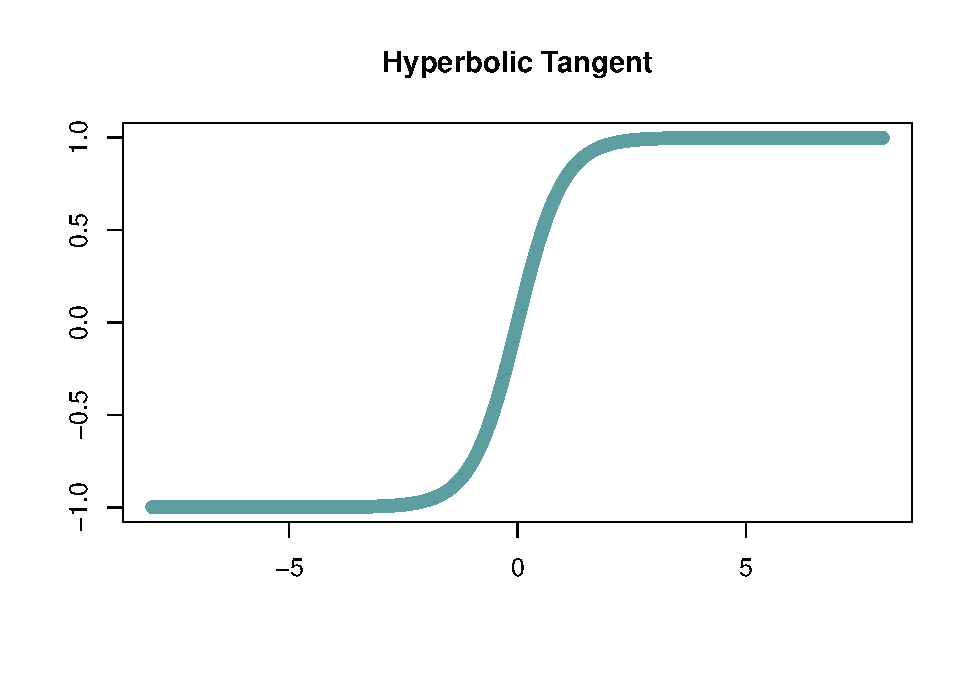
\includegraphics[width=0.5\linewidth]{Figures/other-activation-functions-1.pdf}
    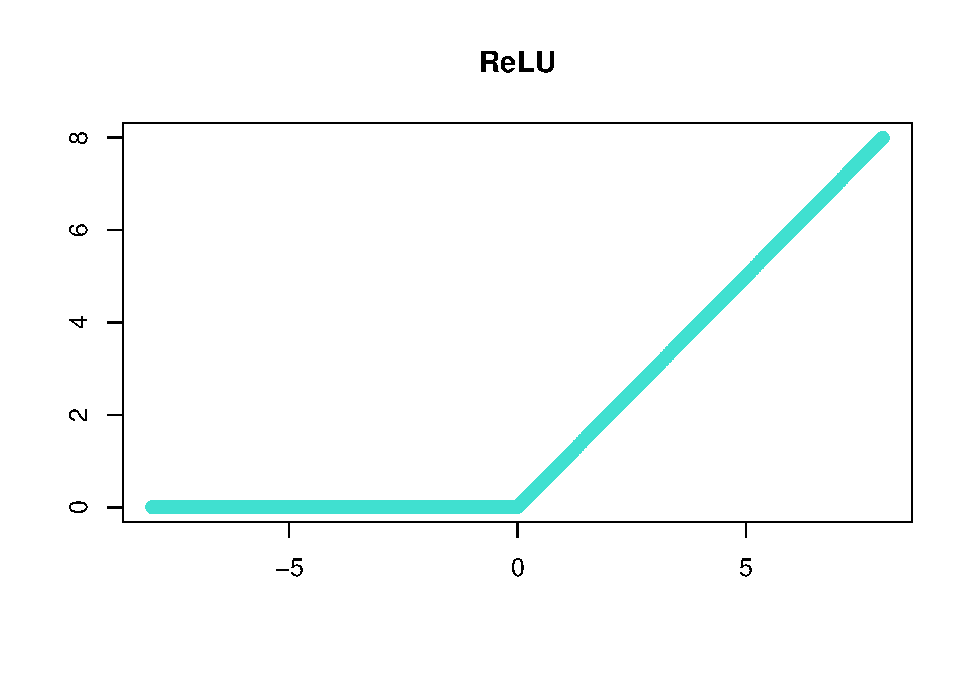
\includegraphics[width=0.5\linewidth]{Figures/other-activation-functions-2.pdf}
    \vspace{-40pt}
 %   \caption{caption}
\end{figure}

Another common activation function is the \textit{rectified linear unit}, or ReLU.  It is defined mathematically as $f(x) = max(0,x)$.  This means that not all neurons will be activated at the same time, which makes ReLU a very useful tool to use in hidden layers to increase efficiency and speed up the learning process. \cite{Goodfellow-et-al-2016} \cite{sharma2017activation}. 
 Variations of ReLU include \textit{leaky ReLU} or \textit{exponential ReLU}, which introduce a means of reducing negative inputs to a very small but still trainable size, rather than zeroing them out entirely.  Similarly, variations of sigmoid, Tanh, and many other activation functions exist and are tested in the interest of improving model efficacy \cite{banerjee2019empirical}.


%------Cost Functions---------

\hypertarget{cost-functions}{%
\subsection{Cost Functions}\label{cost-functions}}

Cost functions, also known as error or loss functions, are defined by taking the negative logarithm of the likelihood function.\cite{bishop2006pattern}  Because of the complexity of neural networks, they have many variations to match specific tasks, and as such many different cost functions can be applied.  To give a comprehensive review of cost functions extends beyond the scope of this thesis.  Instead, some recognizable cost functions that are seen in other models will be described.

For \textbf{regression} tasks, the \textit{Mean Squared Error} loss function is commonly used.

\[
MSE = \frac{1}{N} \sum_{i=1}^N (\hat{y_i} - y_i)
\] Where $\hat{y_i} =$ \(a^{(L)}_i\) is the outcome of a single iteration of forward
propagation and \(y_i\) is the true observation to compare it to.

For \textbf{classification} tasks, variations of the \textit{log-loss} function are applied depending on the task.  Binary classification problems typically use the sigmoid activation function, resulting in the following loss function:

%commenting out general cross-entropy
%$$
%CE = - \sum_{i=1}^N y_i log (\hat{y_i})
%$$

$$
BCE = - \frac{1}{N} \sum_{i=1}^N y_i log (\hat{y_i}) + (1-y_i) log(1-\hat{y_i})
$$

The equation above is often called the \textit{binary cross-entropy} or more simply the \textit{cross-entropy} loss function in literature, but the latter can be misleading.  \textit{Any} loss measured with a negative log likelihood is a cross-entropy between the distributions defined by the training set and that of the model. \cite{Goodfellow-et-al-2016}

for \textbf{multi-class classification} models, the generalized general form of sigmoid known as \textit{softmax} is used as the activation function \cite{bishop2006pattern}.  

$$
P(X) = \frac{e^{\delta_i}}{\sum_j{e^{\delta_j} }}
$$

By the same techniques, the log-loss function generalizes to the following form:
$$
MCE = -\sum_{i=1}^N \sum_{j=1}^M y_{ij} log (\hat{y}_{ij})
$$

All of these are cross-entropy error functions that neural networks use to optimize their parameters by gradient descent.


%---------Gradient Descent---------

\hypertarget{gradient-descent}{%
\subsection{Gradient Descent}\label{gradient-descent}}

The efficiency of a neural network is measured and corrected with each
iteration based on reducing a cost function. This is the same s finding
a local minimum of a function. In a simple case below, given the
function \(f(x) = x^3 + 10x^2\), a local minimum is found by
differentiating the function.

\begin{figure}[H]
    \centering
    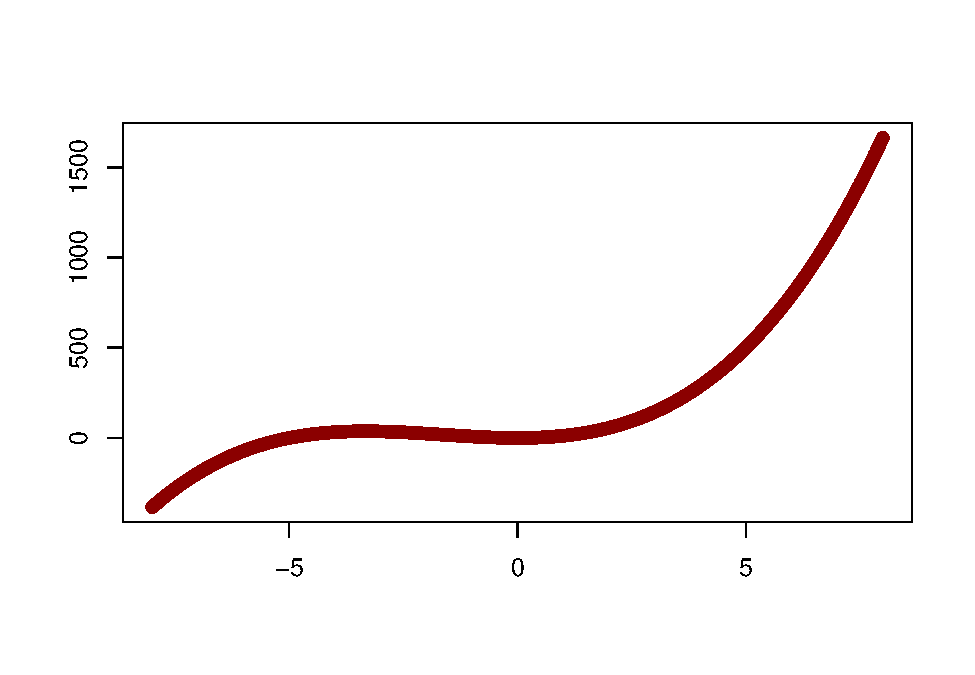
\includegraphics[width = .7\textwidth]{Figures/grad_desc_2D-1.pdf}
\end{figure}

This is ideal when \(x \in \mathbb{R}\), even for
\(x \in \mathbb{R}^2\), but gets more  and more complicated as
dimensionality increases to \(x \in \mathbb{R}^n\). This calls for
another means for finding function extrema (particularly minima).
\textbf{Gradient Descent} is an optimization process by which an extrema is found by
means of iterative computation for high-dimensional functions, making it
intrinsically useful for neural networks to learn.

Figure \ref{grad} displays the three dimensional function $z = \frac{1}{2} x^2 + 4 sin(y)$.  Observing gradient descent in two or three dimensions is perhaps the simplest way to visualize complexity, as biological limitations bar the visualization of higher dimensions.  For computers, however, it is no trouble and the process is the same.  The network propagates forward and determines the outcome error for the vector of weights $w_i$ and biases $b_i$ in the network with the loss function.  It then computes the gradient - the adjustment to every specific $w_i$ and $b_i$ parameter that gives the direction of steepest descent to the loss function - and takes a step in that direction.


\begin{figure}[H]
    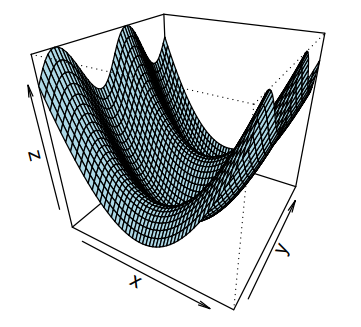
\includegraphics[width = .4\textwidth]{Figures/grad_desc-51.png}
    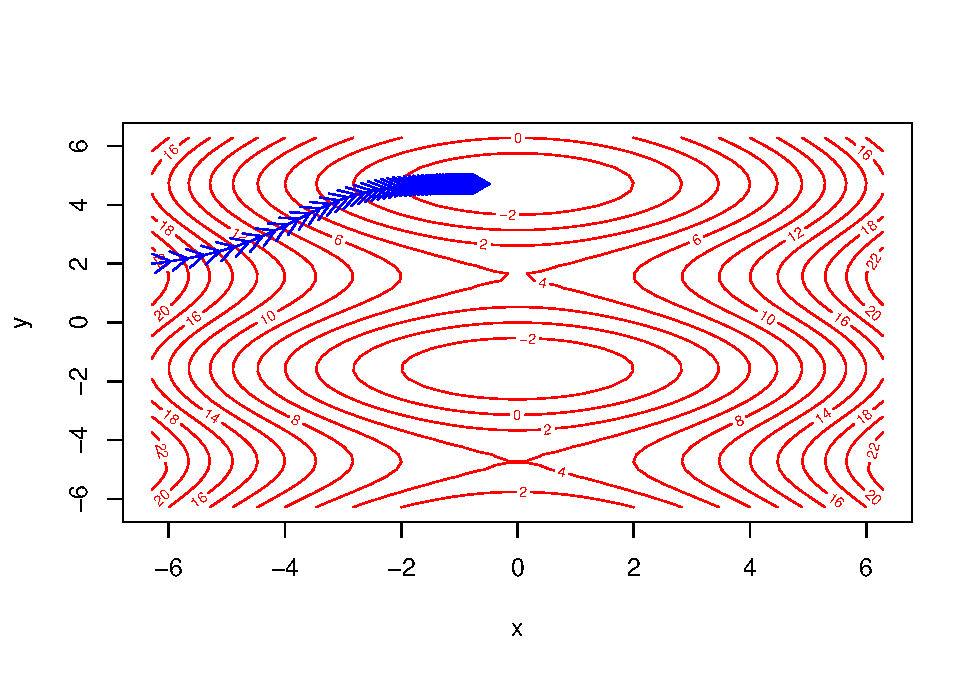
\includegraphics[width = .6\textwidth]{Figures/grad_desc-50.pdf}
    \caption{The function in three dimensions, with a top-down observation that shows the path of gradient descent.  Each blue arrow represents a step.}
    \label{grad}
\end{figure}

%---BACKPROPAGATION---

\hypertarget{backpropagation}{%
\subsection{Backpropagation}\label{backpropagation}}

Backpropagation is the algorithm that drives gradient descent and computes the gradient for high-dimensional derivatives. For a standard neural network, it is composed of the partial derivatives of the cost function with respect to each weight in each layer of the network, and each bias in each layer of the network.

\[
\nabla{C} =
\begin{bmatrix}
\frac{\partial{C}}{\partial{w_1^{(1)}}} & \frac{\partial{C}}{\partial{w_2^{(1)}}} & \cdots & 
\frac{\partial{C}}{\partial{w_i^{(1)}}} \\
\frac{\partial{C}}{\partial{b_1^{(1)}}} & \frac{\partial{C}}{\partial{b_2^{(1)}}} & \cdots & 
\frac{\partial{C}}{\partial{b_i^{(1)}}} \\
\vdots & \vdots & \ddots & \vdots \\
\frac{\partial{C}}{\partial{w_1^{(l)}}} & \frac{\partial{C}}{\partial{w_2^{(l)}}} & \cdots & 
\frac{\partial{C}}{\partial{w_i^{(l)}}} \\
\frac{\partial{C}}{\partial{b_1^{(l)}}} & \frac{\partial{C}}{\partial{b_2^{(l)}}} & \cdots & 
\frac{\partial{C}}{\partial{b_i^{(l)}}} \\
\end{bmatrix}
\] Here, the superscript \(^{(l)}\) denotes the layer of the network and
the subscript \(_i\) denotes a specific parameter within that specific
layer. In this section, the backpropagation calculus will be explained under the example of a \textit{two-layer} network; although the same notation and derivation can be applied to networks of all sizes.
%Here, \(^{(2)}\) will be used to indicate the hidden layer and \(^{(1)}\) the input layer.

The backpropagation algorithm is catered to a specific loss function. In
this example, the loss function is \emph{Mean Squared
Error}. This function takes the difference between the output from the
network and the specified desired output for each observation. To
understand how each parameter that makes up the output must be adjusted,
the algorithm must differentiate every part of it. This is done by use
of the chain rule in calculus. Ultimately, two parameter
differentiations must be computed for each observation in each layer - a
\emph{weight} and a \emph{bias}, as illustrated in the matrix above. By tracing the lineage of influence on the
network's final output backwards
(``back-propagating''), the output is found to be influenced by:

\begin{enumerate}
\tightlist
\item
  an \textit{activation} function in between the hidden layer and the output,
  which itself is influenced by the resulting computation of the hidden layer \emph{weight}, \emph{bias}, and
\item
  \textit{activation} function from the previous layer, which is itself
  influenced by the resulting computation of the previous layer
  \emph{weight}, \emph{bias}, and input layer.
\end{enumerate}

In the two-layer network example, identifying the lineage stops here.  For deeper networks, item (2) is repeated with the term ``input layer'' replaced by ``activation of earlier layers.''


%---partial derivatives with respect to WEIGHT---

\hypertarget{partial-derivatives-with-respect-to-weight}{%
\paragraph{Partial derivatives with respect to
weight}\label{partial-derivatives-with-respect-to-weight}}

The amount to adjust the weight in the \emph{hidden} layer is
represented through use of the chain rule by:
\begin{align*}
\frac{\partial{C}}{\partial{w_i^{(2)}}}    &=  \dfrac{\partial{z_i^{(2)}}}{\partial{w_i^{(2)}}}
     \dfrac{\partial{a_i^{(2)}}}{\partial{z_i^{(2)}}}
     \dfrac{\partial{C}}{\partial{a_i^{(2)}}} \\ 
 &= a_i^{(1)} \sigma'(z_i^{(2)}) 2(a_i^{(2)}-y_i) \end{align*}

where \(a_n^{(1)}\) is the activation for each observation in the first
(input) layer, \(\sigma'(z_i^{(2)})\) is the derivative of the sigmoid
activation function with respect to each observation in the second
(hidden) layer, \(a_i^{(2)}\) is the activation for each observation in
the hidden layer, and \(y_i\) is the vector of actual training values
this network hopes to achieve.

The amount to adjust the weight in the \emph{input} layer is
represented by:

    \begin{align*}
\frac{\partial{C}}{\partial{w_i^{(1)}}}    &= \dfrac{\partial{z_i^{(1)}}}{\partial{w_i^{(1)}}} \dfrac{\partial{a_i^{(1)}}}{\partial{z_i^{(1)}}}  \dfrac{\partial{z_i^{(2)}}}{\partial{a_i^{(1)}}}
     \dfrac{\partial{a_i^{(2)}}}{\partial{z_i^{(2)}}}
     \dfrac{\partial{C}}{\partial{a_i^{(2)}}} \\    
&= x_i \sigma'(z_i^{(1)}) w_i^{(2)} \sigma'(z_i^{(2)}) 2(a_i^{(2)}-y_i) \\
     \end{align*}

where \(x_i\) is the input from our training data,
\(\sigma'(z_i^{(1)})\) is the derivative of the sigmoid activation
function with respect to each observation in the input layer,
\(w_i^{(2)}\) is the vector of weights in the hidden layer, and all else
is the same as is in the previous equation.

%---partial derivatives with respect to BIAS---

\hypertarget{partial-derivatives-with-respect-to-bias}{%
\paragraph{Partial derivatives with respect to
bias}\label{partial-derivatives-with-respect-to-bias}}

The amount to adjust the bias in the \emph{hidden} layer is
represented by: \[
\frac{\partial{C}}{\partial{b_i^{(2)}}}  =  \dfrac{\partial{z_i^{(2)}}}{\partial{b_i^{(2)}}}
     \dfrac{\partial{a_i^{(2)}}}{\partial{z_i^{(2)}}}
     \dfrac{\partial{C}}{\partial{a_i^{(2)}}} \\
\]

Because the bias is a constant, that is
\(\dfrac{\partial{z_i^{(l)}}}{\partial{b_i^{(l)}}} = 1\), the chain-rule
formula simplifies to the following: \[
\frac{\partial{C}}{\partial{b_i^{(2)}}} = 1 \cdot \sigma'(z_i^{(2)}) 2(a_i^{(2)}-y_i) \\
\]

And for the same reasons, the amount to adjust the bias in the \emph{input} layer is
represented by:

    \begin{align*}
\dfrac{\partial{C}}{\partial{b_i^{(1)}}} 
& = \dfrac{\partial{z_i^{(1)}}}{\partial{b_i^{(1)}}} \dfrac{\partial{a_i^{(1)}}}{\partial{z_i^{(1)}}}  \dfrac{\partial{z_i^{(2)}}}{\partial{a_i^{(1)}}}
     \dfrac{\partial{a_i^{(2)}}}{\partial{z_i^{(2)}}}
     \dfrac{\partial{C}}{\partial{a_i^{(2)}}} \\ \nonumber
& = 1 \cdot \sigma'(z_i^{(1)}) w_i^{(2)} \sigma'(z_i^{(2)}) 2(a_i^{(2)}-y_i) \nonumber
    \end{align*}


The preceding demonstration was for a simple shallow network.  In a network with more layers $L$ , the number of equations needed for the full back-propagation increases as well ($2L$ - one for each weight and bias).  As shown, the chain rule increases more and more as lineage tracing gets closer to the initial input layer, resulting in more and more complexity in the calculations.  And because backpropagation is catered to the cost function and the activation function, the specific derivatives calculated will be different as these are changed as well.